\chapter{Results}
\label{chap:results}

The experiment contains 366 evaluation settings with 100,000 sampled
pairs in each. Independent 100,000-pair batches at 186 equal-MI settings
fit the moment references and calibration thresholds. This chapter first
checks the component approximations, then compares the four rejection
rules. All displayed nominal rates divide valid rejections by all
attempts. Brackets around rates and shading in the rejection plots give pointwise
95\% intervals. Reference-rule intervals condition on the independently
fitted degrees of freedom. Complete setting-level rates, denominators
and paired contrasts are supplied in the experiment supplement.

\section{Mean and sampling variance of the estimated MI variance}

The mean approximation and sampling-variance approximation have different
errors. Figure~\ref{fig:redesign-moments} separates them for different-skew
populations at common MI 0.02 nats. A ratio of one indicates agreement.
Solid curves use the population quantities; dashed curves in the middle
row use the mean plug-in sampling-variance prediction. Shading gives
approximate 95\% Monte Carlo intervals for the population-prediction
ratios. The component mean remains inflated after the prediction of its
sampling variance has become reasonably accurate. At \(n=1{,}000\), the population
sampling-variance prediction divided by the observed value ranges from
0.710 to 0.996 across all sizes and margins, while the mean estimate
divided by \(V\) ranges from 1.023 to 4.571. The latter discrepancy is
particularly large for the larger tables.

\begin{figure}[!htbp]
\centering
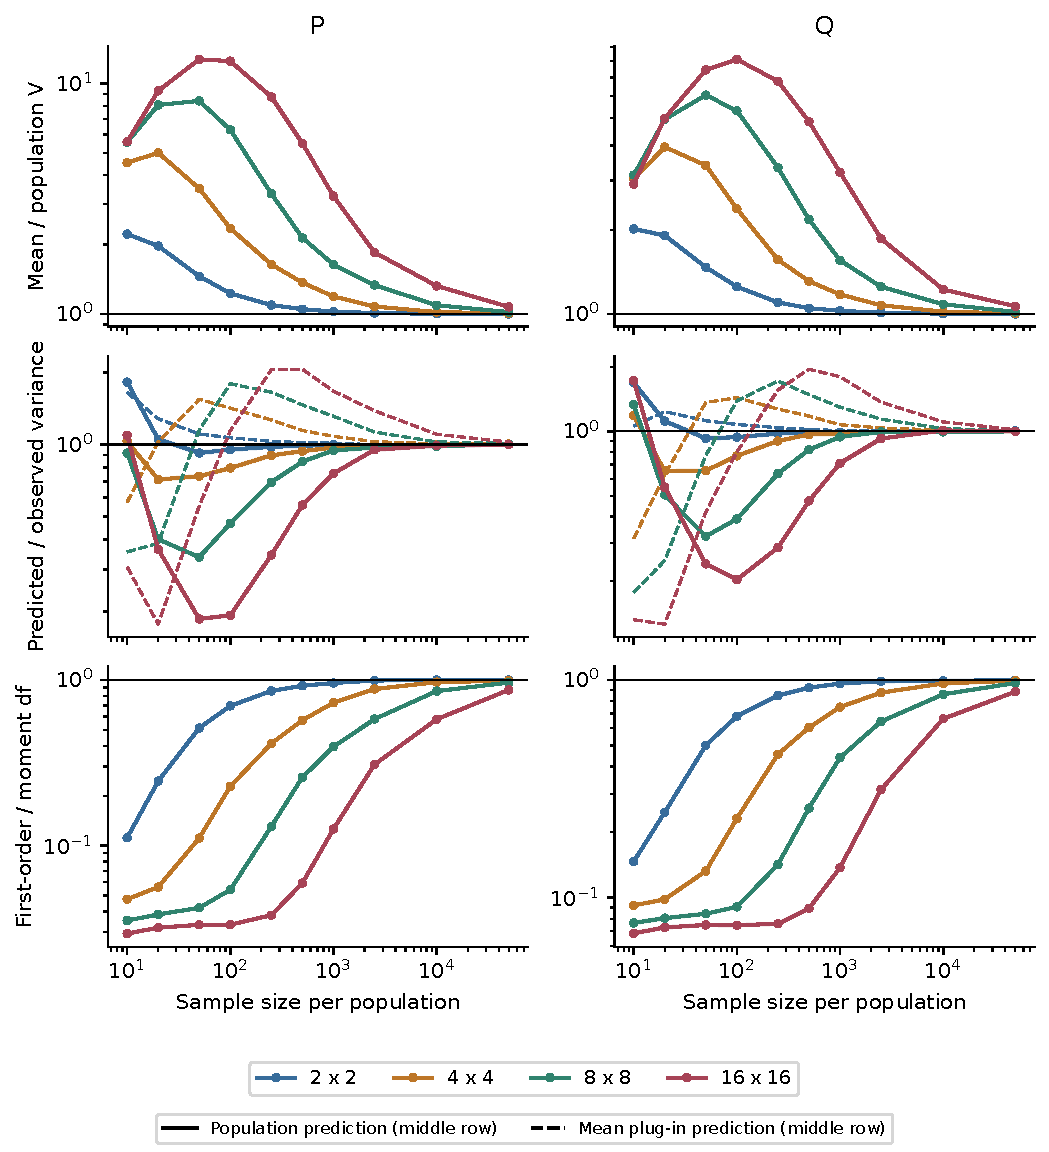
\includegraphics[width=\textwidth,height=.78\textheight,keepaspectratio]{focused_redesign_moments_different_skew.pdf}
\caption{Component approximation ratios under different-skew margins.}
\label{fig:redesign-moments}
\end{figure}

At \(n=50{,}000\), the sampling-variance ratios across the same broad grid
lie between 0.974 and 1.009. Mean ratios range from 1.000 to 1.091, so
small residual mean errors can still affect the degrees of freedom.
The first-order/moment degrees-of-freedom ratios range from 0.862 to 1.006.
Thus increasing sample size improves both approximations, but their
rates of improvement differ. Appendix~\ref{app:additional-results}
provides the uniform and same-skew versions of the figure.

The decomposition in Equation~\eqref{eq:redesign-df-decomposition} explains
this difference. At \(4\times4\), \(n=1{,}000\) and MI 0.02, the
sampling-variance ratios are 0.970 for \(P\) and 0.967 for \(Q\).
Their mean ratios are 1.190 and 1.174. Consequently, the population
first-order degrees of freedom, 15.30 and 13.61, fall below the moment
targets, 21.03 and 18.14. Most of that difference comes from squaring the
mean-ratio contribution, rather than from an inaccurate sampling-variance
prediction. Table~\ref{tab:variance-stability} gives the component values.

\begin{table}[!htbp]
\centering
\small
\setlength{\tabcolsep}{3pt}
\caption{Component moment and degrees-of-freedom comparisons at \(4\times4\), \(n=1{,}000\), different skew.}
\label{tab:variance-stability}
\begin{tabular}{@{}lrrrrrr@{}}
\toprule
MI, pop. & Mean ratio & Pop. var. & Plug-in var. & Mean df & Moment df & FO df\\
\midrule
0.0001, P & 44.939 & 0.047 & 1.965 & 4.86 & 9.12 & 0.10\\
0.0001, Q & 41.996 & 0.052 & 2.142 & 4.44 & 8.63 & 0.09\\
0.02, P & 1.190 & 0.970 & 1.080 & 19.55 & 21.03 & 15.30\\
0.02, Q & 1.174 & 0.967 & 1.072 & 17.00 & 18.14 & 13.61\\
0.05, P & 1.066 & 1.008 & 1.013 & 42.56 & 43.07 & 37.63\\
0.05, Q & 1.057 & 1.031 & 1.029 & 37.59 & 38.61 & 33.50\\
\bottomrule
\end{tabular}

\end{table}

In the table, mean ratio is \(\E\Vhat/V\); the next two columns divide
the population and mean plug-in sampling-variance predictions by the
observed sampling variance of \(\Vhat\). Mean df averages the positive
finite component estimates; all 100,000 estimates are included in each
shown row. Moment df uses the actual sampling moments, while FO df uses
the population first-order formula.

\section{Near independence and the Appendix A.4 predictions}

At MI 0.0001 and \(n=1{,}000\), the quadratic sampling contribution is
large relative to the population first-order variance. The observed
values of \(n\E\Vhat\) are 9.158 for \(P\) and 8.665 for \(Q\),
compared with the Appendix A.4 prediction 9.2. Mean estimated component
degrees of freedom are 4.86 and 4.44, compared with 4.6. The moment
values are 9.12 and 8.63, compared with approximately 9.00. These are
component means and moment targets; a median combined degree of freedom
would answer a different question.

\begin{figure}[!htbp]
\centering
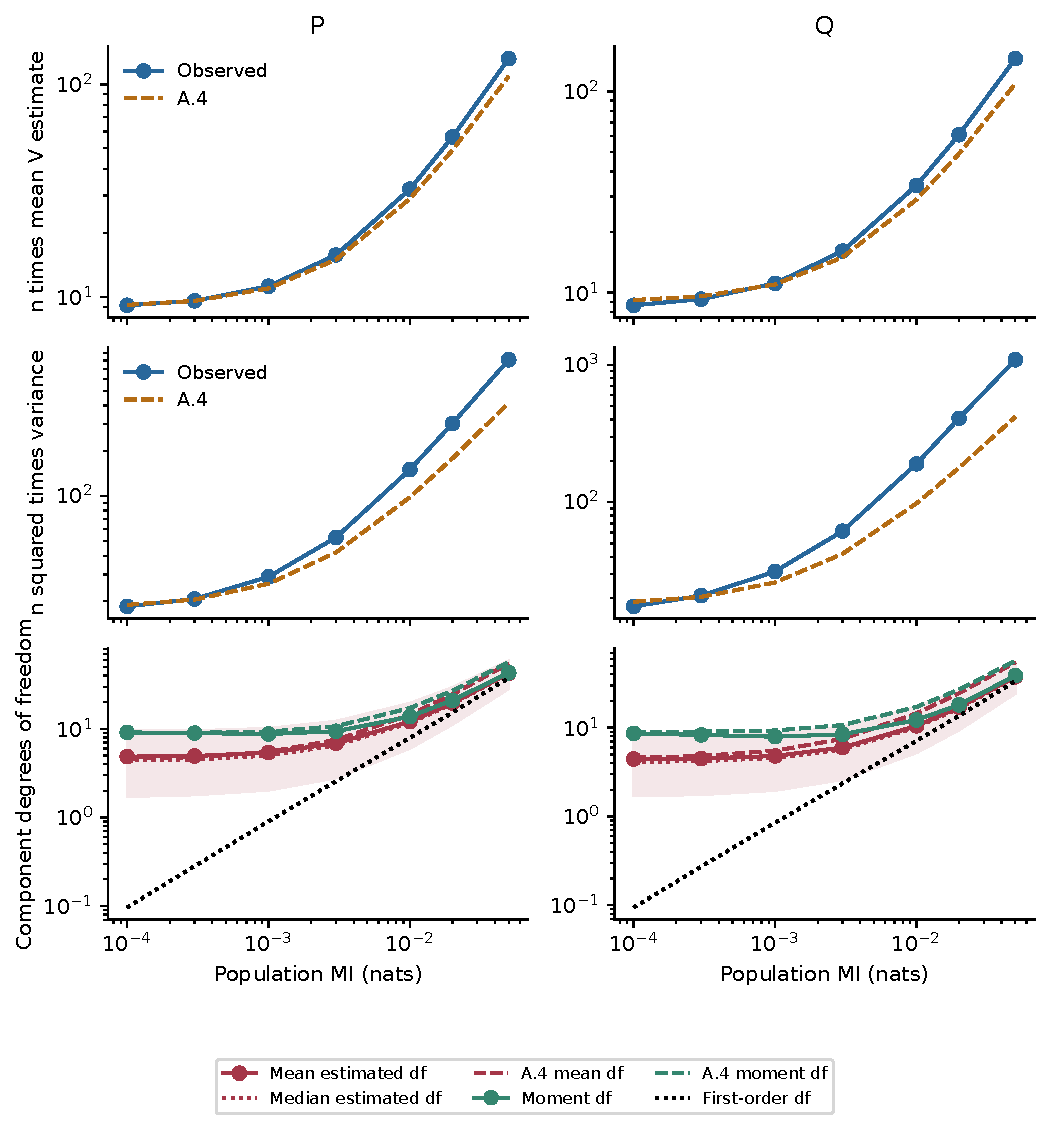
\includegraphics[width=\textwidth,height=.78\textheight,keepaspectratio]{focused_redesign_a4_different_skew_1000.pdf}
\caption{Observed component moments and Appendix A.4 predictions across MI.}
\label{fig:redesign-a4}
\end{figure}

Figure~\ref{fig:redesign-a4} shows how that agreement changes across MI.
The shaded band gives the fifth--95th percentile range of estimated
component degrees of freedom, with their mean and median shown separately.
The first-order prediction for the sampling variance is only about
5\% of the observed value at the smallest MI target. Meanwhile, the
mean plug-in prediction is 1.97 times the observed value for \(P\) and
2.14 times for \(Q\). The local calculation explains the scale of these
errors: the quadratic sampling contribution remains substantial even
though the population first-order degrees of freedom are below 0.1.
At MI 0.02, the population sampling-variance approximation is much more
accurate, while the mean error still lowers the first-order degrees of
freedom relative to the moment target. The mean plug-in variance
predictions remain about 7--8\% above the observed values. Thus the
accuracy of the population variance-sensitivity formula does not eliminate
the error from estimating that sensitivity in each sample.

The scaled mean error varies around
\(d=9\). Across the three margin regimes and seven MI targets, its
observed range is 5.55--8.45 at \(n=100\), 7.50--9.39 at
\(n=1{,}000\), and 7.60--10.19 at \(n=10{,}000\).
Figure~\ref{fig:redesign-mean-bias} displays the changes with population
MI and margins, with 95\% Monte Carlo intervals. The coefficient near
nine explains the persistent upward shift in the component mean for
these \(4\times4\) populations. Its variation with the population table
and sample size determines where a fixed \(d/n\) correction would
leave residual error. Companion comparisons at \(n=100\) and 10,000 are in the appendix.

\begin{figure}[!htbp]
\centering
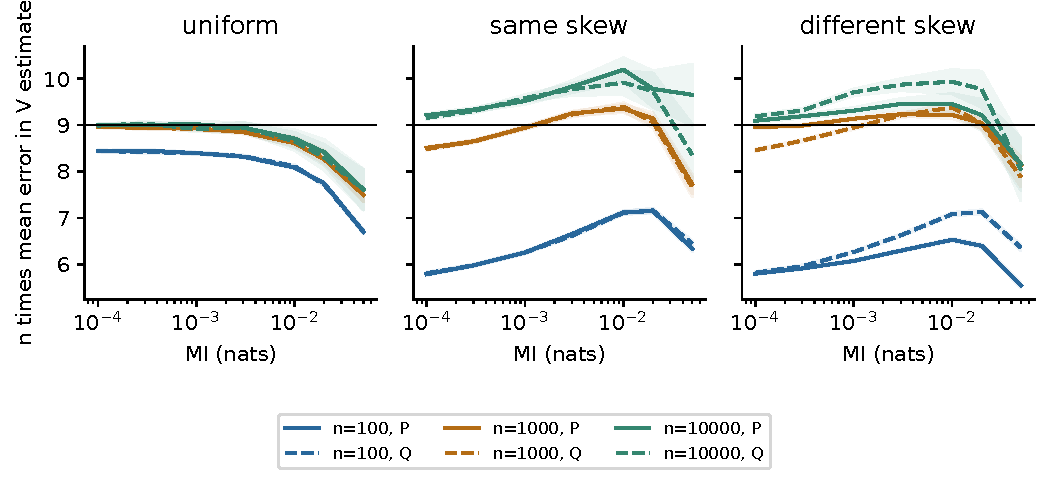
\includegraphics[width=\textwidth]{focused_redesign_mean_bias.pdf}
\caption{Scaled mean error of the variance estimator across population MI.}
\label{fig:redesign-mean-bias}
\end{figure}

\section{False-positive rates across the broad study}

Figures~\ref{fig:redesign-null-uniform} and
\ref{fig:redesign-null-different} compare the four rules at common MI
0.02 nats. Expanded Welch reduces false positives in some small-sample
settings and lowers already-conservative rates in others. The sample-size
comparator often remains close to Normal Wald once sample sizes are
moderate. The moment reference also varies in its calibration, showing
that accurate denominator moments alone do not provide a correctly
calibrated Student \(t\) reference for every population.

\begin{figure}[!htbp]
\centering
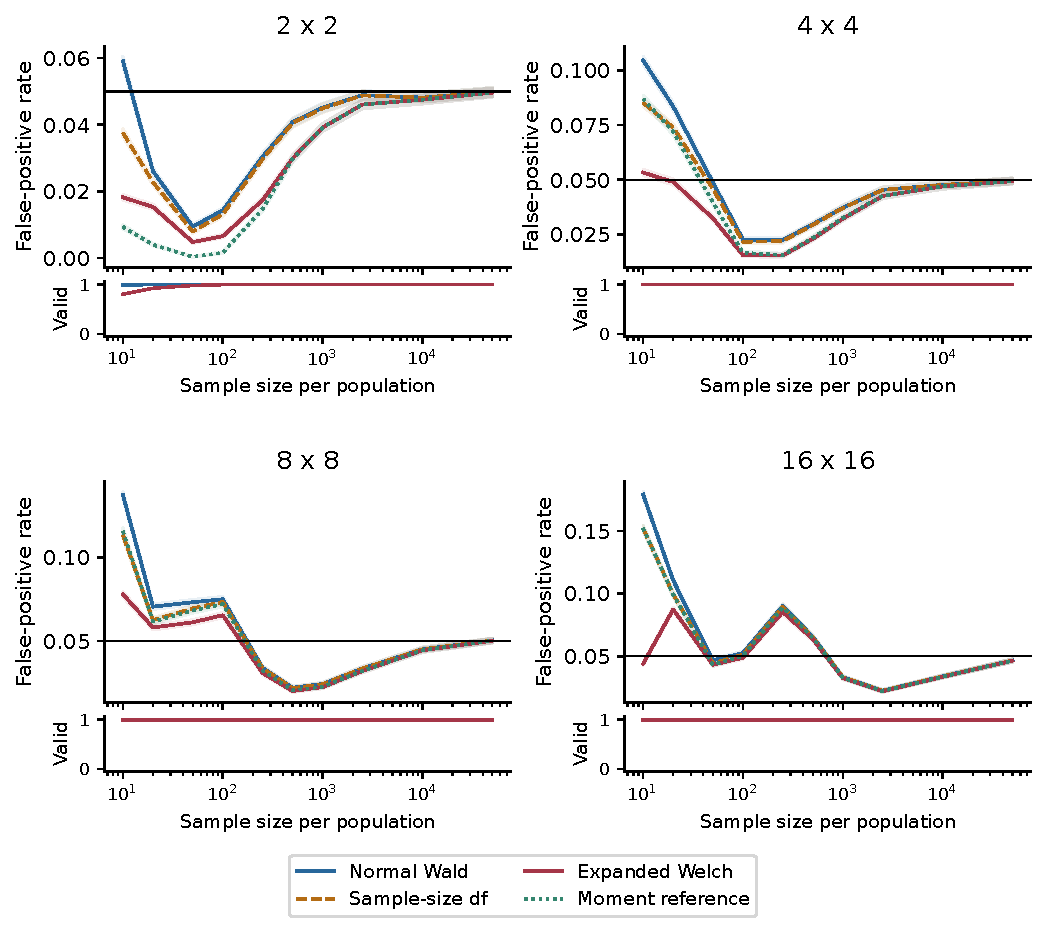
\includegraphics[width=\textwidth]{focused_redesign_null_uniform.pdf}
\caption{False-positive rates under uniform margins.}
\label{fig:redesign-null-uniform}
\end{figure}

\begin{figure}[!htbp]
\centering
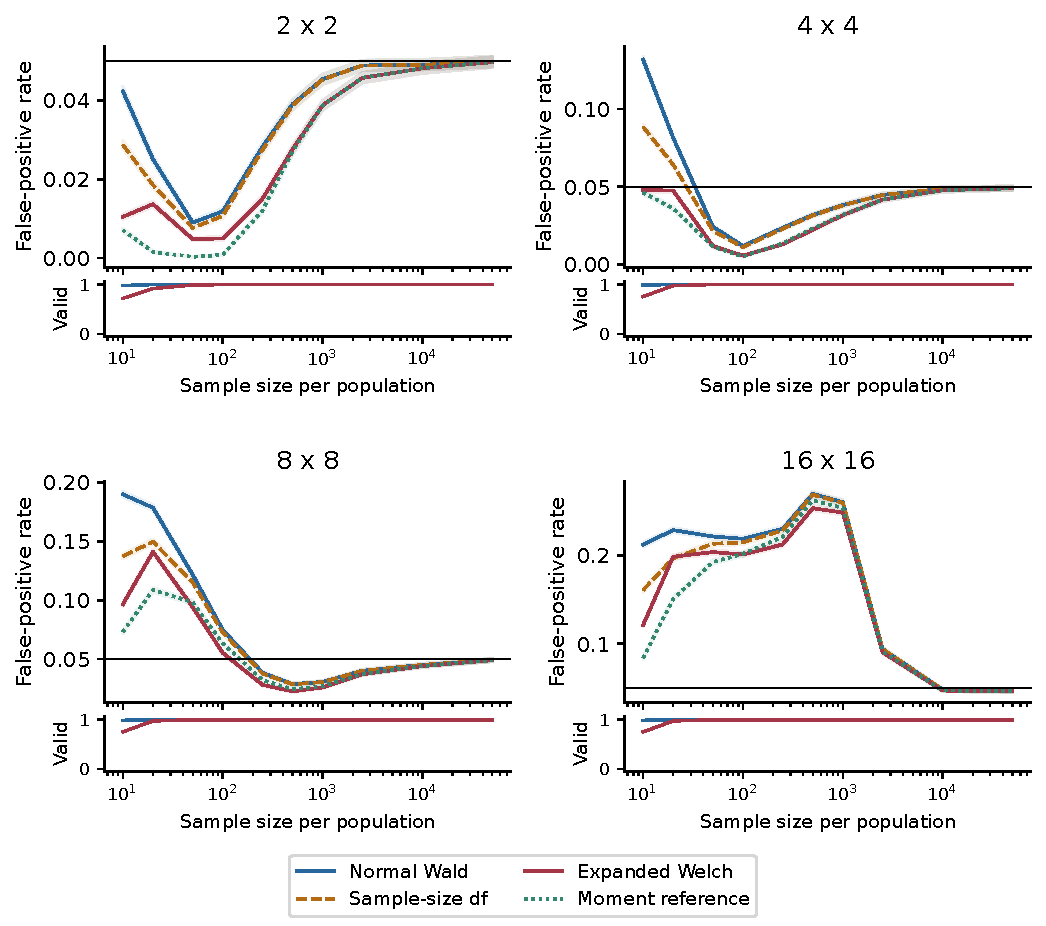
\includegraphics[width=\textwidth]{focused_redesign_null_different_skew.pdf}
\caption{False-positive rates under different-skew margins.}
\label{fig:redesign-null-different}
\end{figure}

The lower panels show the fraction of valid outputs for Normal Wald
and Expanded Welch. The sample-size and fixed-reference rules share
Wald's validity in these settings. Validity is lowest in the
smallest samples: across the 120 settings, the minimum valid fractions
are 0.958 for Normal Wald, the sample-size comparator and the fixed
reference, and 0.631 for Expanded Welch. Their conditional rates and
included counts are reported separately in the supplement.

Across the broad grid, the counts of rates between 4\% and 6\% are
43 for Wald, 41 for the sample-size comparator, 41 for Expanded Welch
and 35 for the fixed reference. Expanded Welch's small-sample improvements
therefore do not extend to uniformly better calibration across the grid.
The different-skew large-table failure and the conservative same-skew
cases explain why a lower rejection rate can improve or worsen agreement
with the 5\% target.

\section{Focus settings and shared estimation failures}

Table~\ref{tab:redesign-case-rates} compares the focus settings with the
matched large-table cases. All four rules are valid on every sampled pair
in these seven settings. At A, Expanded Welch lowers rejection from
0.08352 for Wald and 0.07394 for the sample-size comparator to 0.04897.
The fixed moment reference gives 0.07202. At B, the corresponding rates
are 0.07466, 0.07246, 0.05523 and 0.06331. The B estimate therefore
remains above 5\%, although it is closer than the comparator rates.

\begin{table}[!htbp]
\centering
\small
\setlength{\tabcolsep}{4pt}
\caption{Null rejection rates with pointwise 95\% intervals.}
\label{tab:redesign-case-rates}
\begin{tabular}{@{}lrr@{}}
\toprule
Setting & Normal Wald & Sample-size df\\
\midrule
A & 0.0835 [0.0818, 0.0853] & 0.0739 [0.0723, 0.0756]\\
B & 0.0747 [0.0730, 0.0763] & 0.0725 [0.0709, 0.0741]\\
C & 0.0486 [0.0473, 0.0500] & 0.0486 [0.0473, 0.0500]\\
16, same, 1,000 & 0.0060 [0.0056, 0.0065] & 0.0060 [0.0055, 0.0065]\\
16, same, 10,000 & 0.0438 [0.0426, 0.0451] & 0.0438 [0.0425, 0.0451]\\
16, different, 1,000 & 0.2601 [0.2574, 0.2628] & 0.2595 [0.2568, 0.2622]\\
16, different, 10,000 & 0.0478 [0.0465, 0.0491] & 0.0478 [0.0464, 0.0491]\\
\addlinespace[5pt]
\midrule
Setting & Expanded Welch & Moment reference\\
\midrule
A & 0.0490 [0.0476, 0.0503] & 0.0720 [0.0704, 0.0736]\\
B & 0.0552 [0.0538, 0.0567] & 0.0633 [0.0618, 0.0648]\\
C & 0.0477 [0.0464, 0.0490] & 0.0477 [0.0464, 0.0490]\\
16, same, 1,000 & 0.0053 [0.0048, 0.0057] & 0.0056 [0.0052, 0.0061]\\
16, same, 10,000 & 0.0426 [0.0414, 0.0439] & 0.0427 [0.0415, 0.0440]\\
16, different, 1,000 & 0.2484 [0.2457, 0.2510] & 0.2535 [0.2508, 0.2562]\\
16, different, 10,000 & 0.0468 [0.0455, 0.0482] & 0.0469 [0.0457, 0.0483]\\
\bottomrule
\end{tabular}

\end{table}

\begin{table}[!htbp]
\centering
\small
\setlength{\tabcolsep}{3pt}
\caption{Shared-estimator diagnostics and combined degrees of freedom.}
\label{tab:redesign-case-diagnostics}
\begin{tabular}{@{}lrrrrrr@{}}
\toprule
Setting & Bias/SD & Var. ratio & Corr. & Skew & Median df & Ref. df\\
\midrule
A & 0.003 & 0.827 & 0.006 & 0.002 & 10.61 & 29.70\\
B & 0.870 & 1.535 & -0.177 & -0.052 & 21.12 & 33.34\\
C & 0.000 & 1.010 & -0.091 & -0.013 & 293.23 & 293.98\\
16, same, 1,000 & -0.003 & 1.929 & 0.005 & 0.008 & 78.87 & 142.90\\
16, same, 10,000 & 0.001 & 1.047 & -0.006 & 0.012 & 265.85 & 294.14\\
16, different, 1,000 & 2.058 & 1.938 & -0.129 & -0.008 & 88.51 & 155.70\\
16, different, 10,000 & -0.229 & 1.064 & -0.090 & -0.013 & 299.21 & 329.92\\
\bottomrule
\end{tabular}

\end{table}

In Table~\ref{tab:redesign-case-diagnostics}, bias/SD divides difference
bias by its observed sampling SD; variance ratio divides mean squared
standard error by observed difference variance. Corr. is the correlation
between the difference and its standard error, and skew describes the
difference estimates. These diagnostics describe the shared statistic
without identifying separate causal contributions.

At A, difference bias is negligible, but the estimated variance is only
0.827 of the observed variance. Its median estimated combined degrees of
freedom are 10.61, compared with the fixed moment reference 29.70.
At B, the bias is 0.870 observed SDs and the variance ratio is 1.535.
Its median degrees of freedom are 21.12, compared with reference 33.34.
The lower median degrees of freedom at A and B give larger cutoffs
than the fixed reference on a typical sample, while the sample dependence
of those cutoffs also changes which pairs are rejected. Thus the two
small-sample improvements occur alongside different estimation errors. At C, bias is negligible, the variance ratio is 1.010,
and median and reference degrees of freedom are both about 293--294.

The \(16\times16\), different-skew case at \(n=1{,}000\) remains a
clear failure for all four rules. The difference bias is 0.02985 nats,
about 2.058 observed SDs. Rejection ranges from 0.24836 to 0.26011.
The reference rate is 0.25348 despite its independently fitted moments.
Under the equal-MI null, the estimated difference is centred at
\begin{equation}
 \E(\Deltahat)\approx 0+0.02985=0.02985\text{ nats}.
 \label{eq:redesign-null-bias-shift}
\end{equation}
This shift is large relative to the observed SD of approximately 0.01450
nats. It moves most rejections into the positive tail even though the
population difference is zero.
With same skew, difference bias is negligible and the variance ratio is
1.929; all four rates instead lie between 0.00525 and 0.00604.
The matched populations separate the large difference bias from
conservative behaviour that occurs when the biases cancel. At
\(n=10{,}000\), both skew regimes give much smaller estimation errors
and rates closer to 5\%.

\section{Power at the selected settings}

\subsection{Nominal power}

Figure~\ref{fig:redesign-power} measures power along the fixed paths in
Equation~\eqref{eq:redesign-power-grid}. Expanded Welch has lower nominal
power than the sample-size comparator at A and B. At two null SDs, the
A difference is 0.30993 nats: Expanded Welch rejects 0.35889 of pairs,
compared with 0.38875 for the sample-size comparator and 0.41017 for Wald.
At B, two null SDs is 0.13028 nats, with rates 0.06046, 0.06546 and
0.06773, respectively. These comparisons include the different null
rejection rates shown at zero.

\begin{figure}[!htbp]
\centering
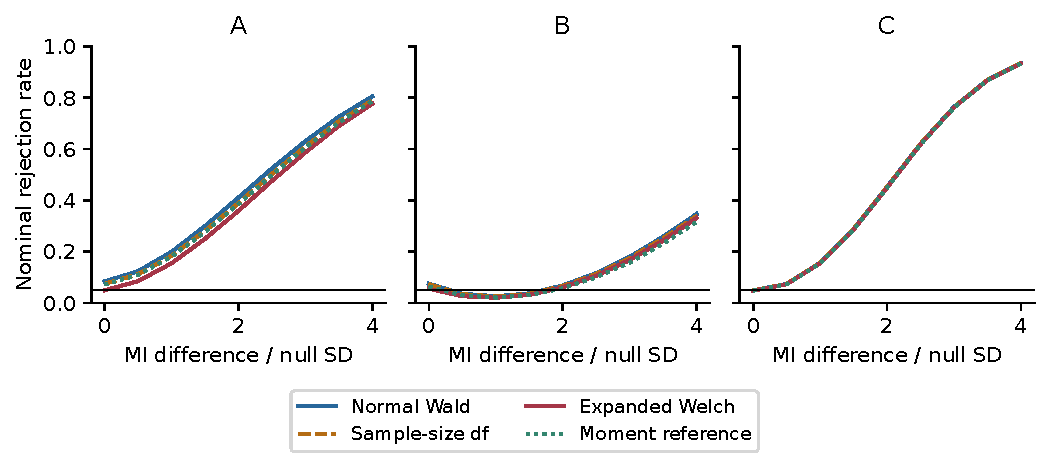
\includegraphics[width=\textwidth]{focused_redesign_power.pdf}
\caption{Nominal power across differences measured in fitted null standard deviations.}
\label{fig:redesign-power}
\end{figure}

B also shows a falling-then-rising rejection curve. Expanded Welch's
rate falls from 0.05523 under the null to 0.01993 at one null SD, before
rising to 0.33075 at four SDs. The true signed difference becomes
negative as \(I(Q)\) increases, initially opposing the positive bias
observed under the null. The larger rejection cutoff does not remove
this distortion of the shared statistic. Direction counts and the
broader large-table curves provide supporting evidence in the appendix.

At C, nominal power differences are small. At two null SDs, or
0.00635 nats, Wald gives 0.45206 and Expanded Welch gives 0.44902.
The paired loss is 0.304 percentage points, with 95\% interval
0.270--0.338. Table~\ref{tab:redesign-power-contrasts} reports paired
comparisons at two null SDs for all three focus settings. These intervals
use the same sampled pairs, so they measure the difference directly.
The calibrated comparison assesses how that difference changes after
matching null rejection.

\subsection{Power after empirical null calibration}

Figure~\ref{fig:redesign-calibrated-power} and
Table~\ref{tab:redesign-calibrated-power} use independent null fitting
to compare rules at approximately 5\% rejection. Null evaluation rates
range from 0.04926 to 0.04994 at A, 0.04961 to 0.04977 at B, and
0.04976 to 0.04981 at C. Wald and the fixed reference have identical
decisions after calibration.

\begin{figure}[!htbp]
\centering
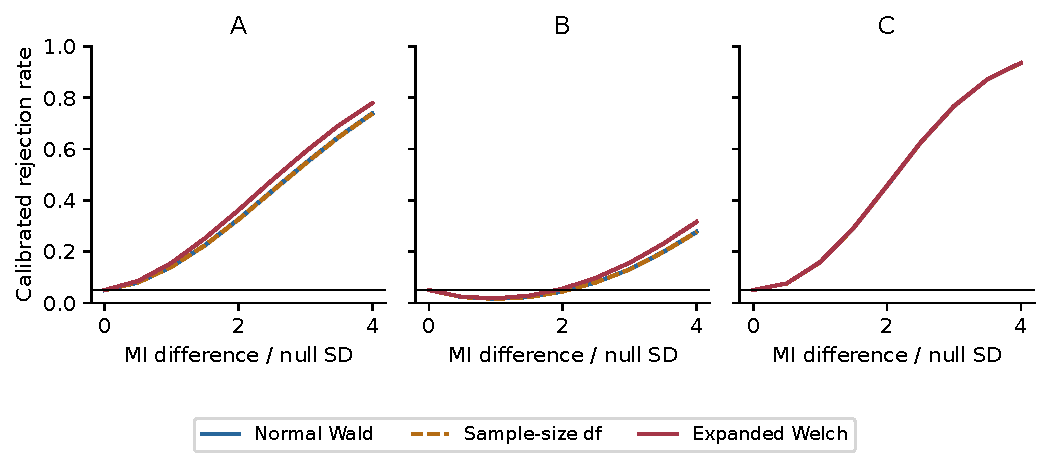
\includegraphics[width=\textwidth]{focused_redesign_power_calibrated.pdf}
\caption{Focused power after independent null calibration; bands show bootstrap uncertainty.}
\label{fig:redesign-calibrated-power}
\end{figure}

\begin{table}[!htbp]
\centering
\small
\caption{Calibrated rejection rates and actual MI differences.}
\label{tab:redesign-calibrated-power}
\begin{tabular}{@{}lrrrr@{}}
\toprule
Setting: SD & Nats & Wald/ref. & Size df & Expanded\\
\midrule
A: 0 & 0.00000 & 0.0493 & 0.0493 & 0.0499\\
A: 1 & 0.15497 & 0.1407 & 0.1403 & 0.1559\\
A: 2 & 0.30993 & 0.3256 & 0.3252 & 0.3614\\
A: 3 & 0.46490 & 0.5441 & 0.5433 & 0.5891\\
A: 4 & 0.61987 & 0.7384 & 0.7377 & 0.7784\\
B: 0 & 0.00000 & 0.0498 & 0.0498 & 0.0496\\
B: 1 & 0.06514 & 0.0154 & 0.0154 & 0.0177\\
B: 2 & 0.13028 & 0.0442 & 0.0441 & 0.0554\\
B: 3 & 0.19541 & 0.1307 & 0.1303 & 0.1564\\
B: 4 & 0.26055 & 0.2766 & 0.2761 & 0.3159\\
C: 0 & 0.00000 & 0.0498 & 0.0498 & 0.0498\\
C: 1 & 0.00317 & 0.1585 & 0.1585 & 0.1588\\
C: 2 & 0.00635 & 0.4561 & 0.4561 & 0.4566\\
C: 3 & 0.00952 & 0.7668 & 0.7668 & 0.7672\\
C: 4 & 0.01270 & 0.9356 & 0.9356 & 0.9358\\
\bottomrule
\end{tabular}

\end{table}

Expanded Welch has higher calibrated power at A. At two null SDs its
rate is 0.36145, compared with 0.32565 for Wald; the paired gain is
3.580 percentage points, with bootstrap 95\% interval 3.295--3.787.
At three SDs, the gain is 4.496 points, with interval 4.230--4.766.
The sample-size comparator remains close to calibrated Wald. These
results show that the sample-dependent MI degrees of freedom can improve
the ordering of evidence along this population path, beyond reducing
the nominal false-positive rate.

B also gives higher calibrated power for Expanded Welch, although its
rejection curve remains distorted. At two SDs, rates are 0.05536 for
Expanded Welch and 0.04424 for Wald, a gain of 1.112 percentage points
with interval 1.028--1.194. At four SDs, the gain is 3.924 points with
interval 3.776--4.151. The initial decline remains after calibration:
matching the null rate does not correct the bias-related power failure.

At C, the calibrated differences are practically small. At two SDs the
rates are 0.45655 and 0.45611, a gain of 0.044 percentage points with
interval 0.013--0.071. The selected one-, three- and four-SD comparisons
also have intervals wholly within the stated one-percentage-point
tolerance. These are pointwise comparisons for the specified populations.
They do not imply a power advantage across untested association patterns.

\begin{table}[!htbp]
\centering
\small
\setlength{\tabcolsep}{3pt}
\caption{Expanded Welch minus each comparator at two null SDs, in percentage points.}
\label{tab:redesign-power-contrasts}
\begin{tabular}{@{}lrrrr@{}}
\toprule
Setting, comparator & Nominal & 95\% interval & Calibrated & 95\% interval\\
\midrule
A, Wald & -5.128 & [-5.265, -4.991] & +3.580 & [+3.295, +3.787]\\
A, size df & -2.986 & [-3.093, -2.879] & +3.629 & [+3.394, +3.865]\\
B, Wald & -0.727 & [-0.780, -0.674] & +1.112 & [+1.028, +1.194]\\
B, size df & -0.500 & [-0.544, -0.456] & +1.123 & [+1.043, +1.210]\\
C, Wald & -0.304 & [-0.338, -0.270] & +0.044 & [+0.013, +0.071]\\
C, size df & -0.296 & [-0.330, -0.262] & +0.044 & [+0.013, +0.071]\\
\bottomrule
\end{tabular}

\end{table}

\section{Supporting construction and allocation comparisons}

\subsection{Changing the association construction}

The four-cell comparison retains the population MI, margins and sample
sizes while concentrating dependence in the first two rows and columns.
It reproduces the main sparse-table failure. At \(16\times16\),
different skew and \(n=1{,}000\), the difference bias is 0.03155 nats,
about 2.023 observed SDs. Wald rejects 0.30958 of pairs and Expanded
Welch rejects 0.29719; the fixed reference gives 0.30129. The copying
rates at the matched setting are 0.26011, 0.24836 and 0.25348. The
size of the error changes with the construction, while severe
over-rejection remains under all four rules.

With same-skew margins at the same size and sample count, the four-cell
null bias is negligible and the variance ratio is 1.659. Its rates are
0.01126 for Wald and 0.01001 for Expanded Welch. As with copying,
matching category frequencies cancels the expected difference bias but
leaves conservative rejection. At \(n=10{,}000\), the four-cell variance
ratios are 1.038 under different skew and 1.022 under same skew, much
closer to one. Table~\ref{tab:redesign-construction} gives the matched
null comparisons, with alternative results in the supplement.

\subsection{Changing the allocation of a fixed sample total}

The allocation comparison retains each \(4\times4\) population pair
and distributes 2,000 observations as \((1000,1000)\), \((400,1600)\)
or \((1600,400)\). Under the different-skew null, Wald's rates are
0.03808, 0.04500 and 0.04524. Expanded Welch gives 0.03162, 0.02927
and 0.02506. Its median degrees of freedom fall from 35.63 under
balance to 14.38 and 11.00 under imbalance, increasing the cutoff and
lowering already-conservative rejection.

At the 0.01-nat alternative, allocating only 400 observations to \(Q\)
reduces Wald power from 0.11483 under balance to 0.05316, and Expanded
Welch power from 0.10260 to 0.03423. The observed SD rises from 0.01173
to 0.01611 nats. Giving \(Q\) 1,600 observations instead gives Wald
power 0.13236 and Expanded Welch power 0.10375. Thus the direction of
imbalance matters because the populations contribute different amounts
of uncertainty and residual bias.

The same-skew null has identical population tables, but unequal sample
sizes leave residual difference biases of approximately \(+0.00129\)
and \(-0.00128\) nats under the two reversed allocations. These signs
reverse with the sample sizes because the MI estimation bias depends
on sample size after the leading correction has been applied.
Table~\ref{tab:redesign-allocation} reports all three allocations under
both nulls and alternatives. The comparison assesses the full method
under imbalance; the identity for combining independent component
moments remains exact.

The earlier check in Appendix~\ref{sec:jackknife-difference-check}
replaces Wald's analytic MI bias correction with a delete-one jackknife,
retaining the existing standard error and standard normal distribution
cutoff. Its 20,000-pair samples provide a separate investigation of
bias correction, rather than an additional rejection
rule. It improves the estimated ordering in the sparse different-skew
alternative while leaving conservative null rejection.

\section{Application to online shopping data}
\label{sec:shoppers-application}

The Online Shoppers Purchasing Intention dataset provides a practical
comparison of month--purchase MI between new and returning visitors
\citep{sakar2018}.
A larger MI means that the month provides more information about whether
a session ends in a purchase. A second comparison uses the weekend
indicator instead of month to examine whether its MI with purchasing
differs between the same visitor groups.

The dataset contains 12,330 sessions, with each session belonging to a
different user according to the source documentation \citep{sakar2018}.
The analysis retains all 1,694 sessions labelled \texttt{New\_Visitor}
and 10,551 labelled \texttt{Returning\_Visitor}, excluding the 85
\texttt{Other} sessions. The outcome is the original Boolean
\texttt{Revenue} variable: true indicates a purchase and false indicates
no purchase. The tests treat the two disjoint visitor groups as independent
samples and the sessions within each group as independent observations.

Each group forms a \(10\times2\) month--purchase count table. The rows
are the ten months recorded in the dataset: February, March, May, June,
July, August, September, October, November and December. The columns
are no purchase and purchase, and each session adds one to its corresponding
cell. Both groups use these same categories, with no smoothing or removal
of zero cells. All ten months occur in both groups, although the new-visitor
February row contains only one session and no purchase. Replacing month
with the Boolean \texttt{Weekend} variable gives a \(2\times2\) table
for each group, with weekday and weekend rows; all four cells are observed.

Both methods use the bias-corrected MI estimates in
Table~\ref{tab:shoppers-application}. For the month tables, the leading
bias correction subtracts \((10-1)(2-1)/(2n)=9/(2n)\) from each plug-in
MI estimate \citep{miller1955,moddemeijer1989};
for the weekend tables, it subtracts \(1/(2n)\). Here \(n\) is the
number of sessions in the relevant visitor group. The estimated
difference is new-visitor MI minus returning-visitor MI for the same
predictor--purchase pair. Normal Wald
compares this difference divided by its standard error with the standard
normal distribution; Expanded Welch uses the same statistic with a
Student \(t\) distribution and estimated degrees of freedom. Both tests
are two-sided at the 5\% level.

\begin{table}[H]
\centering
\caption{MI estimates and two-sample test results for online shopping sessions.}
\label{tab:shoppers-application}
\begingroup
\setlength{\tabcolsep}{4pt}
\begin{tabular}{@{}lrrrrr@{}}
\toprule
 & \multicolumn{2}{c}{Corrected MI (nats)} & & \multicolumn{2}{c}{p-value}\\
\cmidrule(lr){2-3}\cmidrule(l){5-6}
Predictor & New & Returning & \shortstack{Expanded Welch\\degrees of freedom}
 & \shortstack{Normal\\Wald} & \shortstack{Expanded\\Welch}\\
\midrule
Month & 0.004316 & 0.017880 & 26.79 & \(4.71\times10^{-5}\) & \(3.73\times10^{-4}\)\\
Weekend & 0.000664 & 0.000727 & 2.18 & 0.9554 & 0.9601\\
\bottomrule
\end{tabular}
\endgroup
\end{table}

Month has higher estimated MI with purchasing among returning visitors.
The corrected difference is \(-0.013563\) nats, with a standard error of
\(0.003333\) nats, giving
\begin{equation}
  T\approx\frac{-0.013563}{0.003333}\approx-4.069.
  \label{eq:shoppers-month-statistic}
\end{equation}
With 26.79 estimated degrees of freedom, the Student \(t\) distribution gives
a larger p-value than the standard normal distribution, but both tests
reject equal month--purchase MI for new and returning visitors. This
application was selected from an initial exploration
of six comparisons across three public datasets. Accounting for all six
comparisons with Holm's multiple-testing adjustment \citep{holm1979}
gives month p-values of 0.000189 for Normal Wald and 0.00149 for Expanded
Welch, so the conclusion remains unchanged.
Table~\ref{tab:application-holm} lists all six comparisons and their raw
and adjusted p-values.

The weekend comparison gives a different result: the corrected
weekend--purchase MI estimates for new and returning visitors are both
approximately 0.0007 nats. Their difference,
\(-0.000063\) nats, is small relative to the standard error of
\(0.001124\) nats, giving \(T\approx-0.056\). Although Expanded Welch
estimates only 2.18 degrees of freedom, both p-values remain close to one.
Neither test provides evidence that weekend--purchase MI differs between
the visitor groups, but this does not establish that their population MI
values are equal. The small statistic, rather than the degrees of freedom
alone, explains the agreement between the methods here.

Both methods reach the same decisions in this application, although
Expanded Welch returns larger p-values. Its degrees of freedom depend on
how much the estimated MI variances fluctuate relative to their mean
values, so large session counts alone need not make its p-values close
to Normal Wald's.
